\documentclass[border={0.1cm 0.1cm 0.1cm 0.1cm}]{standalone}  %E,S,W,N

\usepackage{amssymb}
\usepackage{amsmath}
\usepackage{tikz}
\usetikzlibrary{calc}	%for centerarc

%NB: modified code for ellipses instead of circles
\def\centerarc[#1](#2)(#3:#4:#5 and #6) {\draw[#1] ($(#2)+({#5*cos(#3)},{#5*sin(#3)})$) arc (#3:#4:#5 and #6);}

\begin{document}
	
	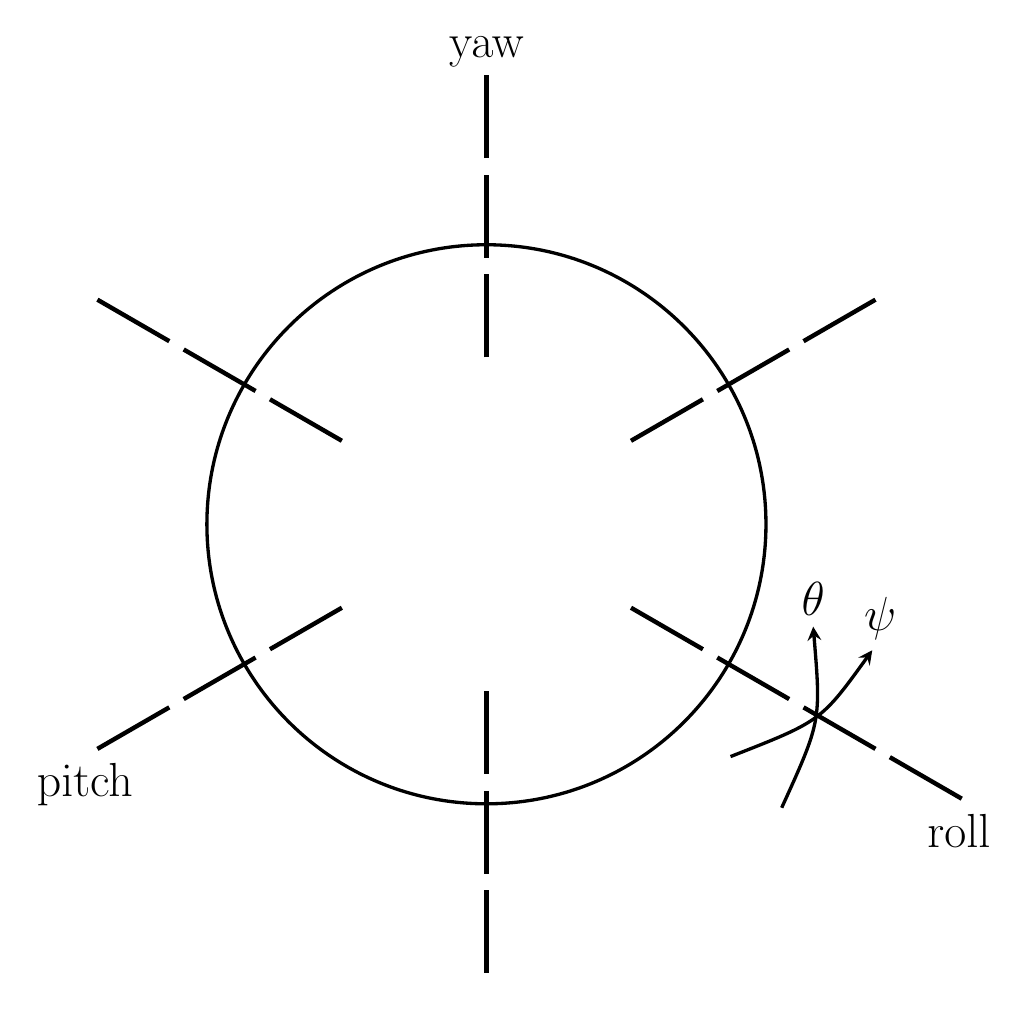
\begin{tikzpicture}[very thick]
	%ELLIPSES
	\draw (0,0) circle (3.55cm);
	%
	\centerarc[dash pattern=on 11 off 3](0,0)(0:180:3.55 and 2.1)
	\centerarc[](0,0)(180:360:3.55 and 2.1)
	%
	\centerarc[dash pattern=on 11 off 3,rotate=120](0,0)(0:180:3.55 and 2.1)
	\centerarc[rotate=120](0,0)(180:360:3.55 and 2.1)
	%
	\centerarc[dash pattern=on 11 off 3,rotate=-120](0,0)(0:180:3.55 and 2.1)
	\centerarc[rotate=-120](0,0)(180:360:3.55 and 2.1)
	
	%CURVED ARROWS
	\centerarc[->,>=stealth](0,4.5)(405:110:1 and 0.6)
	\centerarc[->,>=stealth,rotate=120](0,4.5)(405:110:1 and 0.6)
	\centerarc[->,>=stealth,rotate=-120](0,5.5)(405:110:1 and 0.6)
	
	%STRAIGHT LINES
	\foreach \i in {-1,...,3} \draw[rotate={60*\i},ultra thick,dash pattern=on 30 off 6] (0,2.12)--(0,5.9);
	\draw[rotate={60*4},ultra thick,dash pattern=on 30 off 6] (0,2.12)--(0,7);
	
	%LABELS
	\node at (0,6) {\LARGE yaw};
	\node at (-5.1,-3.3) {\LARGE pitch};
	\node at (6,-3.9) {\LARGE roll};
	%
	\draw[->,>=stealth] (3.75,-3.6) .. controls (4.25,-2.5) .. (4.15,-1.3) node[above] {\LARGE $\theta$};
	\draw[->,>=stealth] (3.1,-2.95) .. controls (4.25,-2.5) .. (4.9,-1.6) node[above,xshift=1mm] {\LARGE $\psi$};
	\end{tikzpicture}
	
\end{document}